\section{Discussion}

With the experimental data established, we now turn to a critical evaluation of the parallel architecture. This discussion interprets the observed scaling efficiency and hardware-bound bottlenecks. Furthermore, it addresses the algorithmic and theoretical limitations of our current tileset design, and outlines actionable strategies for future optimization, specifically targeting the reduction of MPI communication overhead.

\subsection{Comment on the Results}
Looking at the obtained results, we observe that we achieve an optimal speedup as it seems to go develop linearly with the number of processes.
Taking a closer look, even looking at the efficiency statistic, we observe that actually up to 16 processes the algorithm scales super-linearly: this can be explained by the fact that the processes are running on shared local memory and cache and this brings serious advantages.

Once the number of processes cannot be executed on a single socket, as the CAPRI infrastructure only contains cpu's with 16 cores, we observe slowdowns provoked by the time spent in the communication procedures: we see that from P16 to P25 the time pent in synch goes up by about 2 seconds.

This slowdown can be directly observed in the Efficiency study: from P25 the efficiency of our usage of the processors goes down since they spend a lot of time just waiting for the communications. Even with this slowdown the implementations remains efficient in the usage of the different processes since it stops at arount 60\% of usage. 

\subsection{Further Notes on $\texttt{Maze}_{16}$}

In its current formulation, $\texttt{Maze}_{16}$ does not guarantee the global
connectivity of the generated maze: the WFC algorithm may produce multiple
disconnected corridor components that are locally valid with respect to the
tile constraints but do not form a single traversable structure.

Enforcing global connectivity requires a two-phase post-processing pipeline,
which represents the standard approach in procedural content generation for
maze-like environments \cite{atlantis2018pcg}:

\begin{description}
    \item[Flood fill:] Once generation is complete, a flood fill traversal is
    performed from an arbitrary passable cell. All cells reachable from the
    starting point are marked as belonging to the main connected component;
    all remaining passable cells are identified as isolated regions. This step
    runs in $\mathcal{O}(N)$ time and provides a complete map of the
    connectivity structure of the generated maze.

    \item[Selective regeneration:] Isolated regions identified by the flood
    fill are discarded and their cells reset to the virgin state. The WFC
    algorithm is then re-run locally on these regions, with the boundary
    constraints inherited from the surrounding already-collapsed cells, until
    a fully connected configuration is produced.
\end{description}

While this pipeline may appear inefficient due to the potential for repeated
local regenerations, it is consistent with the state of the art in
constraint-based procedural content generation, where post-processing
validation passes are standard practice to enforce global structural
properties that lie outside the scope of local tile
constraints.

The connectivity guarantee was deliberately excluded from the present
implementation: the post-processing pipeline does not interact with the
parallel design in any meaningful way, and no parallel formulation of the
connectivity enforcement step was identified that would not introduce
sufficient synchronization overhead to degrade performance below the
sequential baseline. Although some interesting ideas came up during discussions.

\subsection{Tileset Generalization}
The implementation is designed to accommodate future extensions to additional 
tile sets. The central requirement for any such extension is that the chosen 
tile set must satisfy $\Delta_{prop} < L$, so that propagation remains confined 
within the mask boundary. While this property is amenable to direct proof for 
structured sets such as $\texttt{Maze}_{16}$, no general decision procedure 
exists for establishing $\Delta_{prop}$ for an arbitrary tile set.

This undecidability is a consequence of a deeper result in the theory of Wang 
tiles. Wang conjectured in 1961 that any finite set of tiles capable of tiling 
the plane could do so periodically \cite{wang1961}. His student Robert Berger 
refuted this conjecture in 1966 by proving the undecidability of the domino 
problem that is, no algorithm can determine in general whether a given finite 
tile set admits a valid tiling of the plane constructing as a corollary the 
first known aperiodic tile set \cite{berger1966}. The minimal such set was 
subsequently identified by Jeandel and Rao, who proved that no aperiodic set 
of Wang tiles exists with fewer than 11 tiles or fewer than 4 
colors (where colors are the different types of border connections) \cite{jeandel2015aperiodic}.

As a consequence, no graph-theoretic or structural analysis of an arbitrary 
tile set can decide whether it satisfies the propagation bound required by 
the parallel algorithm. The most practical approach for validating a candidate 
tile set remains probabilistic: a Monte Carlo analysis over a representative 
sample of configurations provides an empirical estimate of $\Delta_{prop}$, 
sufficient for practical purposes even in the absence of a formal proof.


\subsection{Optimizing Data Transfer via Spiral Trajectory and Caching}

Currently, the 9-round mask sliding mechanism evaluates the $3 \times 3$ local grid in a standard row-major order. While geometrically conflict-free, this approach introduces discontinuous jumps in the focal pivot for each round with index multiple of 3.

This overhead can be mitigated by adopting a continuous, spiral-like traversal path together with chunk caching. 
\begin{figure}[H]
\definecolor{m_green}{rgb}{0.1, 0.6, 0.4}
\definecolor{m_red}{rgb}{0.9, 0.2, 0.3}
\centering
\begin{subfigure}[b]{0.48\textwidth}
\centering
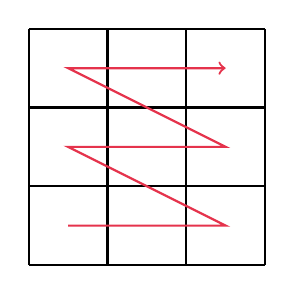
\begin{tikzpicture}
    \draw[step=1cm, black, thick] (0,0) grid (3,3);
        
    \draw[->, thick, m_red] (0.5,0.5) -- (2.5,0.5) -- (0.5,1.5) -- (2.5,1.5) -- (0.5, 2.5) -- (2.5, 2.5);

\end{tikzpicture}
\caption{Row Major}
\end{subfigure}
\begin{subfigure}[b]{0.48\textwidth}
\centering
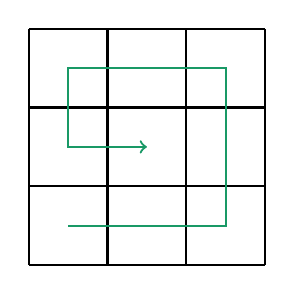
\begin{tikzpicture}
    \draw[step=1cm, black, thick] (0,0) grid (3,3);
        
    \draw[->, thick, m_green] (0.5,0.5) -- (2.5,0.5) -- (2.5,2.5) -- (0.5,2.5) -- (0.5, 1.5) -- (0.5, 1.5) -- (1.5, 1.5);

\end{tikzpicture}
\caption{Spiral}
\end{subfigure}
\caption{The comparison between the current (a) and future (b) round path.}
\end{figure}

Under this configuration, the spatial offset between the pivot at round $k$ and round $k+1$ is strictly bounded to a Chebyshev distance of 1. If we represent the set of chunks covered by the mask at step $k$ as $M_k$, a continuous trajectory maximizes the spatial intersection between consecutive iterations:

$$ |M_k \cap M_{k-1}| = 6 $$

If we introduce a local memory cache for incoming MPI halo data, the node no longer needs to query the full boundary region. Instead, it only needs to fetch the newly exposed frontier:

$$ \Delta M_k = |M_k \setminus M_{k-1}| \le 3 $$

By sliding a cached boundary window, the system requests at most 3 new chunks per iteration. This structural optimization would significantly reduce the overall volume of asynchronous \texttt{MPI\_Sendrecv} data transfers, directly addressing the communication and gathering bottlenecks observed in the strong scaling analysis.


